% Document: Bachelor Thesis: Minimal Problem Solver Generator
% Author: Pavel Trutman

\documentclass[msc]{cmpthesis}
\usepackage[czech,english]{babel}
\usepackage[utf8]{inputenc}
\usepackage{indentfirst}
\usepackage{enumitem}
\usepackage{textcomp}
\usepackage{algorithm}
\usepackage{algpseudocode}
\usepackage{amsmath}
\usepackage{amssymb}
\usepackage{forloop}

\usepackage{subcaption}
\usepackage{pdflscape}
\usepackage{multirow}
\usepackage{dirtree}

% for better verbatim environment
\usepackage{fancyvrb}

% to inlucude pdf pages
\usepackage{pdfpages}

% list of symbols and abbreviations
\usepackage[acronym,nonumberlist,style=long,sort=def]{glossaries}
\setlength{\glsdescwidth}{0.6\linewidth}
\setlength{\glspagelistwidth}{0.4\linewidth}
\renewcommand*{\glsgroupskip}{}
\newcommand{\Acronym}[2]{\newacronym{#1}{#1}{#2}}
\Acronym{cl$(S)$}{Closure of the set $S$}
\Acronym{dom $f$}{Domain of the function $f$}
\Acronym{Dom $f$}{cl(dom $f$)}
\Acronym{int $S$}{Interior of the set $S$}
\newacronym{P}{$\mathcal{P}^n$}{Cone of positive semidefinite $n\times n$ matrices}
\newacronym{S}{$\mathcal{S}^n$}{Space of $n\times n$ real symmetric matrices}
\Acronym{tr$(A)$}{Trace of the matrix $A$}
\newacronym{i-th element of x}{$x^{(i)}$}{$i$-th element of the vector $x$}

\makeglossaries

% algorithmic macros and settings
\newcounter{counter}
\renewcommand{\algorithmicrequire}{\textbf{Input:}}
\renewcommand{\algorithmicensure}{\textbf{Output:}}
\algdef{S}[IF]{IfML}[1]{\algorithmicif\ #1}
\newcommand{\StatexIndent}[1][1]{
  \Statex\forloop{counter}{0}{\value{counter} < #1}{\hskip\algorithmicindent\hskip-0.25em}
}

\startThesisInfo
\title{Semidefinite Programming for Geometric Problems in Computer Vision}
\author{Pavel Trutman}
\CMPAdvisor{Ing. Tom\'a\v s Pajdla, PhD.}
\CMPReportNo{}
\CMPAcknowledgement{\centering }

\CMPEmail{pavel.trutman@fel.cvut.cz}
\CMPDocumentURL{http://cmp.felk.cvut.cz/~trutmpav/master-thesis/thesis/thesis.pdf}
\stopThesisInfo

% ============================== your definitions (abbreviations etc.)
\DeclareMathOperator{\lcm}{lcm}
\DeclareMathOperator{\LM}{LM}

\setitemize{noitemsep,topsep=0.2cm,parsep=0.2cm,partopsep=0pt,leftmargin=1cm}
\setenumerate{noitemsep,topsep=0.2cm,parsep=0.2cm,partopsep=0pt,leftmargin=1cm}

% =========================================================== settings
\graphicspath{{images/}}

% ========================================================== text body
\begin{document}

\cleardoublepage\def\thepage{\roman{page}}\setcounter{page}{3}

% thesis assignment as required by FEE, CTU
%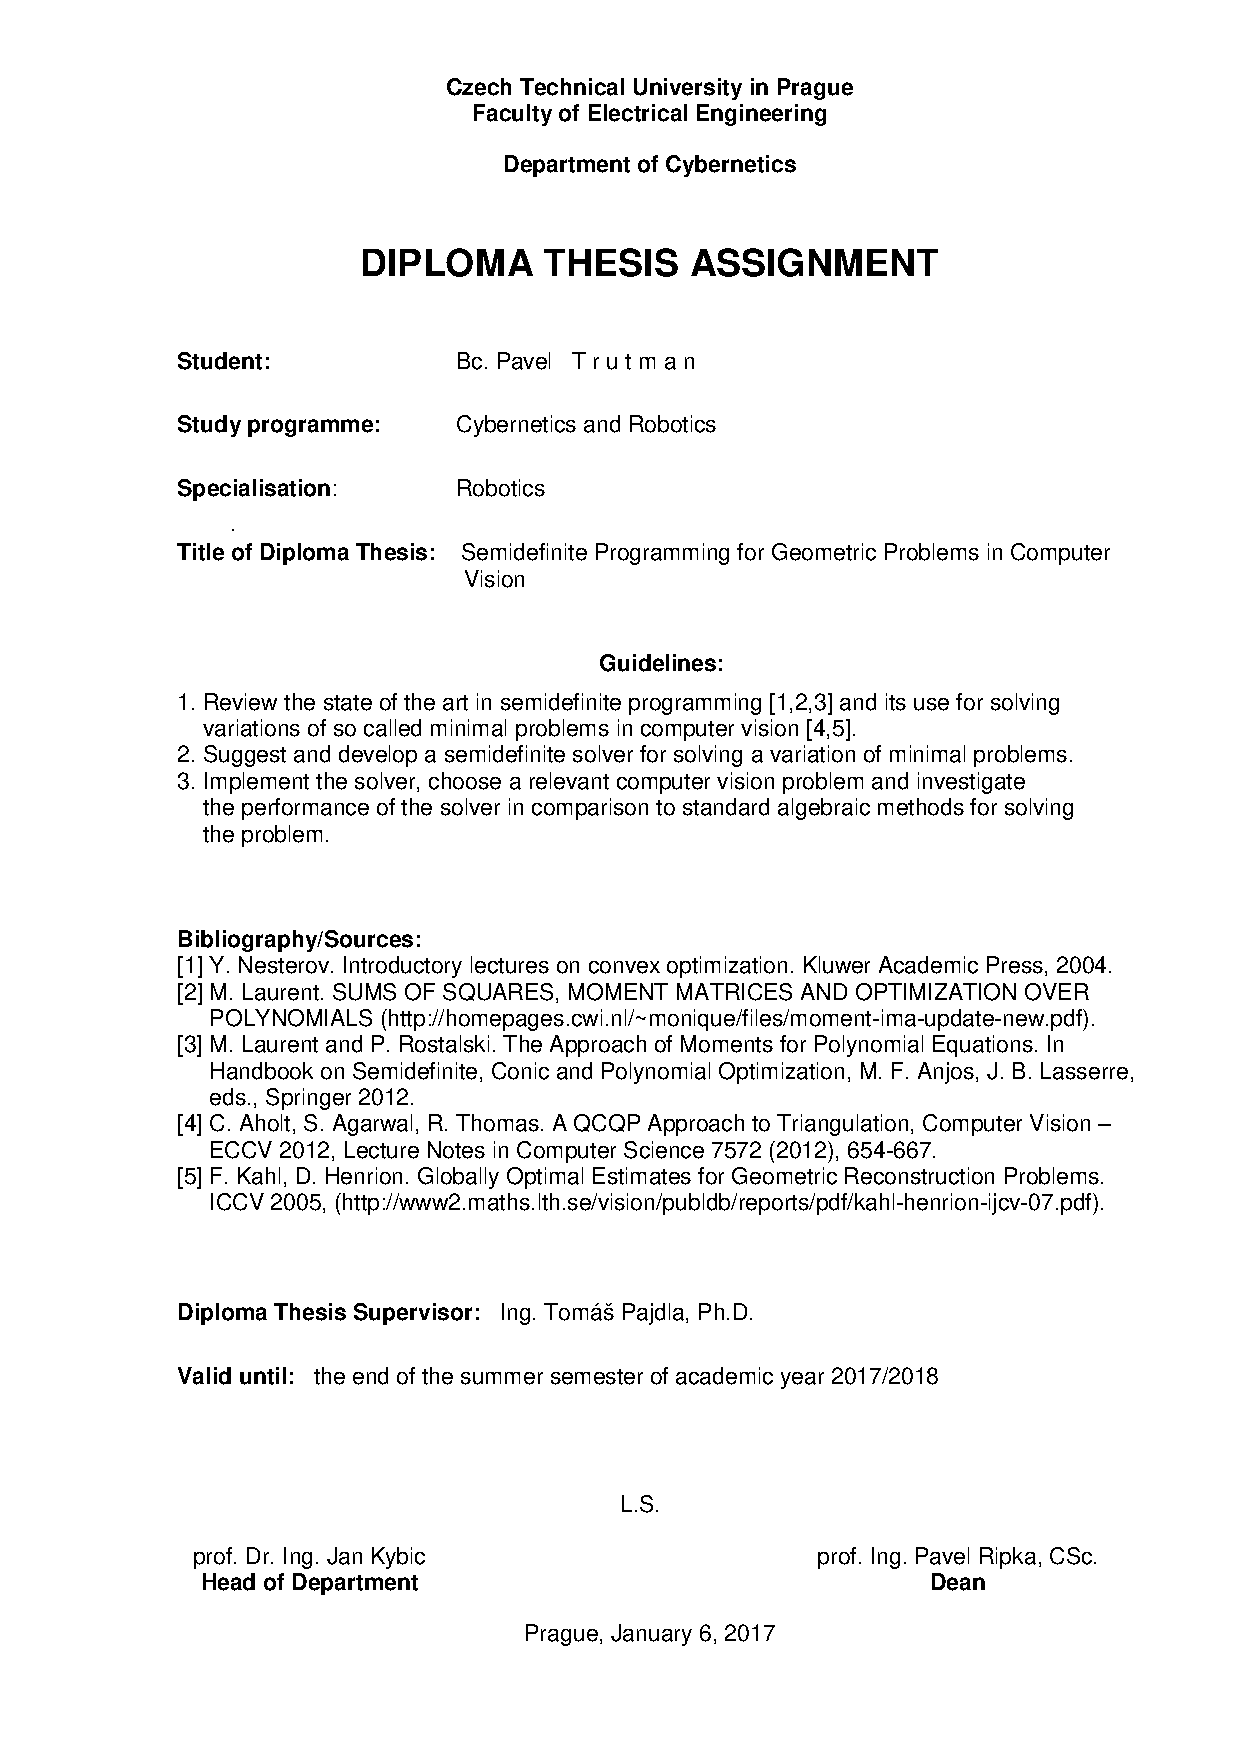
\includepdf[pages={1}]{pdfs/assignment-ENG.pdf}
%\includepdf[pages={1}]{pdfs/assignment-CZE.pdf}

\mbox{}\vfill

{\let\clearpage\relax\par \chapter*{Acknowledgements}}
I would like to express my thanks to my advisor Tom\'a\v s Pajdla for his guidance and valuable advices, which enabled me to finish this thesis.
I would also like to thank Didier Herion for introducing me into semidefinite programming and polynomial optimization techniques and for his useful discussion and comments to my work.
Special thanks go to my family for all their support.

\clearpage
\mbox{}\vfill

{\let\clearpage\relax\par \chapter*{Author's declaration}}
I declare that the presented work was developed independently and that I have listed all sources of information used within it in accordance with the methodical instructions for observing the ethical principles in the preparation of university theses.

%{\let\clearpage\relax\par \chapter*{Prohl\'a\v sen\'i autora pr\'ace}}
%Prohla\v suji, \v ze jsem p\v redlo\v zenou pr\' aci vypracoval samostatn\v e a \v ze jsem uvedl ve\v sker\'e pou\v zit\'e informa\v cn\'i zdroje v souladu s Metodick\'ym pokynem o dodr\v zov\'an\'i etick\'ych princip\r u p\v ri p\v r\'iprav\v e vysoko\v skolsk\'ych z\'av\v ere\v cn\'ych prac\'i.

\vskip3cm
\begin{tabular}{lp{1cm}c}
  Prague, date \makebox[4cm]{\dotfill} &  & \makebox[5cm]{\dotfill}\\
  & & Signature
\end{tabular}

\clearpage
\chapter*{Abstract}
Many problems in computer vision lead to polynomial systems solving.
The state of the art algebraic methods for polynomial systems solving are able to efficiently solve the systems over complex numbers, but the non-real solutions are then discarded, as they are not solutions of the original geometric problems.
On this purpose, we review and implement the moment method for polynomial systems solving, which solves the problems over real numbers directly.
We show that the moment method is applicable to the minimal problems from computer vision geometry.
For that, we give description of the calibrated camera pose problem and of the calibrated camera pose with unknown focal length problem.
We compare our implementation of the moment with the state of the art methods on these two selected minimal problems on real 3D scene.

Moreover, we review and implement a method for solving polynomial optimization problems, which can extend the moment method with inequality constraints.
This method uses Lasserre's hierarchies to find the optimal values of the original optimization problems.
We compare the performance of our implementation with the state of the art methods on synthetically generated polynomial optimization problems.

Since the semidefinite programs solving is a key element in the moment method and the polynomial optimization methods, we review and implement an interior-point algorithm for semidefinite programs solving.
We compare the performance of our implementation with the state of the art methods on synthetically generated semidefinite programs.

\paragraph{Keywords:}
computer vision, polynomial systems solving, polynomial optimization, semidefinite programming, minimal problems

\begin{otherlanguage}{czech}
\chapter*{Abstrakt}
Mnoho problémů v počítačovém vidění vede na řešení systémů polynomiálních rovnic.
Současné metody na řešení systémů polynomiálních rovnic jsou schopny řešit tyto systémy v oboru komplexních čísel, ale následně jsou nereálná řešení vyřazena, protože ta nejsou řešeními původních geometrických problémů.
Z tohoto důvodu prozkoumáme a implementujeme metodu momentů pro řešení systémů polynomiálních rovnic, která řeší tyto problémy přímo v oboru reálných čísel.
Ukážeme, že metoda momentů je použitelná na minimální problémy z geometrie počítačového vidění.
Proto popíšeme problém nalezení polohy kalibrované kamery a problém nalezení polohy kalibrované kamery s neznámou ohniskovou vzdáleností.
Na těchto dvou vybraných minimálních problémech a reálné 3D scéně porovnáme naší implementaci metody momentů se sou\-čas\-ný\-mi metodami.

Dále prozkoumáme a implementujeme metodu na řešení polynomiálně optimalizačních problémů, která může rozšířit metodu momentů o omezení s nerovnostmi.
Tato metoda využívá Lasserrových hierarchií k nalezení optimálních hodnot původních optimalizačních problémů.
Na synteticky generovaných polynomiálně optimalizačních prob\-lé\-mech porovnáme výkon naší implementace se současnými metodami.

Protože řešení semidefinitních programů je klíčovým elementem metody momentů a metod polynomiální optimalizace, prozkoumáme a implementujeme algoritmus vnitřních bodů na řešení semidefinitních programů.
Na synteticky generovaných semidefinitních problémech porovnáme výkon naší implementace se současnými metodami.

\paragraph{Klíčová slova:}
počítačové vidění, řešení polynomiálních systémů, polynomiální optimalizace, semidefinitní programování, minimální problémy
\end{otherlanguage}

\clearpage
\cleardoublepage\def\thepage{\arabic{page}}\setcounter{page}{1}
\tableofcontents\pagestyle{headings}
\listofalgorithms

\glsaddall
\printglossary[type=acronym,title=List of Symbols and Abbreviations]

\chapter{Introduction}
In geometry of computer vision, many problems are formulated as systems of polynomial equations.
The state of the art methods are based on polynomial algebra, i.e.\ on Gr\"obner bases and multiplication matrices computation.
Contrary to this approach, this work applies non-linear optimization techniques to solve the polynomial systems, which is a novel idea in the field of geometry of computer vision.
Moreover, the application of the optimization techniques allows us to enrich the polynomial systems with polynomial inequalities or to solve polynomial optimization problems, i.e.\ optimizing a polynomial function with given polynomial constraints.

\section{Motivation}
Object recognition and localization, reconstruction of 3D scenes, self-driving cars, film production, augmented reality and robotics are only few of many applications of geometry of computer vision.
Thus, one would like to solve geometric problems efficiently, since these problems often have to be solved in real-time applications.
Typical geometric problems from computer vision are the minimal problems, which arise when estimating geometric models of scenes from given images.
To be able to solve these problems computationally, they are often represented by systems of algebraic equations.
Hence, one of the issues of computer vision is, how to solve systems of polynomial equations efficiently, which is the scope of this work.

The polynomial systems obtained from the geometric problems are often not trivial, but usually consist of many polynomial equations of high degree in several unknowns.
From that reason, general algorithms for polynomial systems solving are not efficient for them, and therefore special solvers have been developed for different problems to solve these problems efficiently and robustly.
Previously, these solvers were handcrafted, which is quite time demanding process that has to be done for each problem from scratch.
Then, the process was automated by automatic generators \cite{autogen, larsson}, which automatically generate efficient solver for a given type of the polynomial system.
These solvers obtain the Gr\"obner basis of the system and then construct the multiplication matrix, from which solutions are extracted by eigenvectors computation.
The side effect of this approach is that some non-real solutions often appear amongst real solutions, which are not solutions to the original geometric problem.
Since the computation of the non-real solutions takes time, a method which would find real solutions only may be faster than the contemporary approach.

Some of the arisen systems may be overconstrained.
Such systems have a solution when solved on precise data using precise arithmetic, but they have no solution when solved on real noisy data.
However, these systems may be transformed into optimization problem by relaxing some of the constrains and by minimizing the error of these constraints.
Therefore, an efficient polynomial optimization method may prove useful for overconstrained systems.

\section{Contributions}
To solve polynomial systems over real numbers only, we apply the moment method introduced by J. B. Lasserre et al.
This method uses hierarchies of semidefinite programs to find a Gr\"obner basis of real radical ideal constructed from the ideal generated by the given polynomials.
Then, a multiplication matrix is constructed and solutions are obtained from it.
In this case, the multiplication matrix should have smaller size than a multiplication matrix obtained from the automatic generator, which can save some computation time.
We implement this method in Python and MATLAB and examine its properties on several minimal problems from geometry of computer vision on real 3D scenes.
We show that this method is applicable on problems from computer vision.

The second contribution of this work is, that we describe and review a method for polynomial optimization problems.
This method solves hierarchies of semidefinite programs to find the optimal value.
An application of this method can, for example, be a solver of overconstrained polynomial systems.
We implement our own implementation of this method in Python and compare it to the state of the art methods on synthetic polynomial optimization problems.

Since semidefinite programs solving is a key element in both previously mentioned methods, we review and describe an interior-point method for semidefinite programs solving.
To be able to use this method in implementations of the moment method and the polynomial optimization method, we implement this interior-point method in Python.
To verify our implementation we compare it to the state of the art semidefinite solvers on synthetic semidefinite programs.

\section{Thesis structure}
In this work, we first review an interior-point method for semidefinite programs solving.
To do so, general properties of self-concordant functions and barriers need to be introduced, since they are key elements in convex optimization.
Then, a specialized barrier function for semidefinite programming will be described.
%The knowledge of semidefinite programming is important for us, since it plays crucial role in polynomial optimization techniques described later in the text.
We describe our implementation of the semidefinite programs solver and compare it to the state of the art methods.

Secondly, we focus on polynomial optimization.
After an introduction to polynomial algebra and moment matrices, we describe and implement a method, which solves polynomial optimization problems by relaxations of semidefinite programs.
Then, we review the moment method and describe its implementation in Python.
%The moment method allows us to solve systems of polynomial equations over real numbers.

To compare the implementation of the moment method to the state of the art methods, we introduce two minimal problems from computer vision on which we perform the experiments.
The minimal problems are the estimation (i) of the calibrated camera pose and (ii) of the calibrated camera pose with unknown focal length.
We show that our implementation of the moment method is applicable to these selected geometric problems from computer vision.


\chapter{Conclusions}
In this work, we have reviewed and implemented interior-point method for semidefinite programs solving.
In the experiments on synthetic semidefinite programs we have verified the correctness of the implementation and we have compared it to the state of the art methods.
The results showed that our implementation is significantly slower than the state of the art methods, but an efficient semidefinite programs solver was not a goal of this work.
However, the goal was to understand the implemented method, so we can now exploit its advantages and minimize the effects of its disadvantages when applied in polynomial optimization methods.
In \refsec{SDP:sa} we have shown that typically only few iterations of \refalg{SDP:scb:pf} are enough to get a good approximation of the optimal point.

Furthermore, we have focused on polynomial optimization.
We have implemented a method, which uses hierarchies of semidefinite programs to solve the original non-convex problem.
The new implementation has been compared to the state of the art methods on synthetically generated polynomial optimization problems.
From the results can be seen that our implementation is slower than the state of the art methods, which is mainly because of the inefficient SDP solver, which is the most time consuming part of the algorithm.

The main contribution of this work is the review and implementation of the moment method for polynomial systems solving.
The advantage of this method is that it allows us to find only real solutions of polynomial systems, which can save some computation time.
We have successfully applied this method to some minimal problems from geometry of computer vision, which is a novel idea in the field of computer vision.

To see the performance of the implementation of the moment method on some real problems, we have described two simple minimal problems (namely P3P and P3.5Pf problems) from geometry of computer vision, which we have tested on real 3D scene.
We have found out that for the P3P problem there is about 40 \% of non-real solutions, which need not be computed.
For the P3.5Pf problem it is about 50 \% of all solutions.
The comparison with the algebraic solvers showed that the moment method is applicable on the minimal problems, i.e.\ that the estimation errors of the camera poses and the focal lengths are comparable to the results of the state of the art methods.
The main drawback of the moment method is the computation time, which is significantly higher compared to the algebraic solvers generated by the automatic generator \cite{autogen}.

\section{Future work}
We have seen that the described moment method can be applied on minimal problems from computer vision, but due to its slow computation time it is not comparable to the algebraic methods.
The performance can be improved by many ways.

Firstly, it showed up that the semidefinite programs constructed inside the moment method have typically no feasible strictly interior point.
Therefore, the interior-point algorithm we have implemented in \refcha{SDP} can not be used to find a feasible point from the relative interior.
In this work, we have solved this issue by solving another semidefinite program \refeqb{POP:sol:SDP_tau}.
Different approach can be to implement another SDP solver, which would use an infeasible interior-point method.
Another solution to this issue may bring a method called facial reduction \cite{facial}.
This method is able to find a reduced version of the original problem by solving a sequence of easier semidefinite programs.
Using this method we would be able to remove the superfluous dimensions of the SDP problem, which causes that then the problem is solvable by an interior-point method and moreover the size of the problem is reduced, and therefore some computation time can be saved.

Secondly, it is possible that the idea of automatic generators \cite{autogen, larsson} could be transformed to the optimization world, i.e.\ that for a given problem we would be able to generate a parametrized solver that would solve the problem efficiently for a given value of parameters of the problem.
This idea is proposed in \cite{SDPstability}.
The authors suggest that if we found out that the SDP relaxation is tight for a given value of parameters, and therefore solves the problem correctly, then under some sufficient conditions the relaxation is tight even for small perturbation of the parameters.
Moreover, from histograms in \reffig{app:P3P:histRelax} and \reffig{app:P35Pf:histRelax} we can see that typically one relaxation order prevails over the others.
Therefore, it would make sense not to start from the minimal possible relaxation order in \refalg{POP:sol:alg}, but to solve the problem only for one given relaxation order that would be known in advance.

Although we were unable to show that the moment method can beat the algebraic methods in computation time, there might be a problem on which the moment method will be faster.
Such a problem would have probably a lot of non-real solutions and only few real solutions, so the moment method could benefit from its advantages.
If such a problem would be found, the moment method could be included amongst the state of the art methods for polynomial systems  solving in computer vision.

Another advantage of usage optimization methods for polynomial systems solving, which we have not shown in this work, is that overconstrained systems can be solved by them.
An overconstrained system can be solved in precise arithmetic, but typically it has no solution when solved on real noisy data in floating-point arithmetic.
But the constraints of such problems can be relaxed and the errors of them minimized, and then the optimization techniques as described in \refsec{POP:opt} can be applied.
We have not provided such an experiment in this work, but it would be nice to find a problem, on which this approach would be applicable and to see, how this approach is performing compared to the state of the art approaches.

In this work, we have provided one implementation for polynomial optimization problems solving (\refsec{POP:opt}) and a different one for solving polynomial systems (\refsec{POP:sol}).
This is because of the evolution of this work.
But since both these methods are based on hierarchies of semidefinite programs, it makes sense to implement one universal algorithm, which would be able to solve both tasks.
The advantages are obvious.
We would be able to add constraints in form of polynomial equations to the polynomial optimization problems \refeqb{POP:opt:polmin}, which currently allows only polynomial inequality constraints.
On the other hand, we would be able to introduce polynomial inequalities into the systems of polynomial equations and eliminate some solutions by this approach.
This would lead to smaller multiplication matrices, and therefore to faster eigenvector computations.
A typical example from minimal problems from computer vision may be to impose positivity on focal lengths.


\appendix
\chapter{Contents of the enclosed CD}

\dirtree{%
 .1 /.
   .2 thesis/ \DTcomment{\begin{minipage}[t]{8cm}folder with files related to the thesis\end{minipage}}.
     .3 data/ \DTcomment{\begin{minipage}[t]{8cm}dataset for the experiments\end{minipage}}.
     .3 sources/.
     .4 scripts/ \DTcomment{\begin{minipage}[t]{8cm}scripts performing the experiments\end{minipage}}.
     .3 thesis.pdf \DTcomment{\begin{minipage}[t]{8cm}digital copy of the thesis\end{minipage}}.
   .2 polyopt/ \DTcomment{\begin{minipage}[t]{8cm}the polyopt package\end{minipage}}.
     .3 polyopt/ \DTcomment{\begin{minipage}[t]{8cm}sources of the polyopt package\end{minipage}}.
     .3 tests/ \DTcomment{\begin{minipage}[t]{8cm}unit tests\end{minipage}}.
     .3 demoPOPSolver.py \DTcomment{\begin{minipage}[t]{8cm}polynomial optimization demo\end{minipage}}.
     .3 demoPSSolver.py \DTcomment{\begin{minipage}[t]{8cm}polynomial systems solving demo\end{minipage}}.
     .3 demoSDPSolver.py \DTcomment{\begin{minipage}[t]{8cm}semidefinite programming demo\end{minipage}}.
     .3 setup.py \DTcomment{\begin{minipage}[t]{8cm}install script\end{minipage}}.
   .2 momentMethod/ \DTcomment{\begin{minipage}[t]{8cm}MATLAB implementation of the moment method\end{minipage}}.
     .3 solve.m \DTcomment{\begin{minipage}[t]{8cm}MATLAB function implementing the moment method\end{minipage}}.
}


\bibliographystyle{plain}
\bibliography{citations}{}

\end{document}
